%%%%%%%%%%%%%%%%%%%%%%%%%%%%%%%%%%%%%%%%%%%%%%%%%%%%%%%%%%%%%%%
%
% Welcome to Overleaf --- just edit your LaTeX on the left,
% and we'll compile it for you on the right. If you open the
% 'Share' menu, you can invite other users to edit at the same
% time. See www.overleaf.com/learn for more info. Enjoy!
%
%%%%%%%%%%%%%%%%%%%%%%%%%%%%%%%%%%%%%%%%%%%%%%%%%%%%%%%%%%%%%%%
\documentclass{beamer}
\usepackage{tikz}
\usetheme{CambridgeUS}
\usecolortheme{beaver}
\usepackage{listings}
%%%%%%%%%%%%%%%%%%%%%%%%%%%%%%%%%%%%%%%%%%%%%%%%%%%%%%%%%%%%%%%%%%%%%%%%%%%%%%%%%%%%%%%%%%%%%%%%%%%%%%%%%%%%%%%%%%%%%%%%%%%%%%%%%%%%%%%%%%%%%%%%%%%%%%%%%%%%%%%%%%%%%%%%%%%%%%%%%%%%%%%%%%%%%%%%%%%%%%%%%%%%%%%%
%CODE
\usepackage{listings}
\usepackage{xcolor}

\definecolor{codegreen}{rgb}{0,0.6,0}
\definecolor{codegray}{rgb}{0.5,0.5,0.5}
\definecolor{codepurple}{rgb}{0.58,0,0.82}
\definecolor{backcolour}{rgb}{0.95,0.95,0.92}

\lstdefinestyle{mystyle}{
    backgroundcolor=\color{backcolour},   
    commentstyle=\color{codegreen},
    keywordstyle=\color{teal},
    numberstyle=\tiny\color{codegray},
    stringstyle=\color{purple},
    basicstyle=\ttm\tiny,
    breakatwhitespace=false,         
    breaklines=true,                 
    captionpos=b,                    
    keepspaces=true,                 
    numbers=left,                    
    numbersep=5pt,                  
    showspaces=false,                
    showstringspaces=false,
    showtabs=false,                  
    tabsize=2
}

\lstset{style=mystyle}
%%%%%%%%%%%%%%%%%%%%%%%%%%%%%%%%%%%%%%%%%%%%%%%%%%%%%%%%%%%%%%%%%%%%%%%%%%%%%%%%%%%%%%%%%%%%%%%%%%%%%%%%%%%%%%%%%%%%%%%%%%%%%%%%%%%%%%%%%%%%%%%%%%%%%%%%%%%%%%%%%%%%%%%%%%%%%%%%%%%%%%%%%%%%%%%%%%%%%%%%%%%%%%%%

\title[Projet 2.2] %optional
{Projet 2.2}
\subtitle{NoDEfr-2, une norme pour la description des offres de formation}
\author{Aurélia Fontaine \and Alexia Gross}



\date % (optional)
{Soutenance, Mai 2021}


%End of title page configuration block
%------------------------------------------------------------
%The next block of commands puts the table of contents at the 
%beginning of each section and highlights the current section:

\AtBeginSection[]
{
  \begin{frame}
    \frametitle{Table of Contents}
    \tableofcontents[currentsection]
  \end{frame}
}
%------------------------------------------------------------
\begin{document}
\frame{\titlepage}
%---------------------------------------------------------
%Highlighting text


%%%%%%%%%%%%%%%%%%%%%%%%%%%%%%%%%%%%%%%%%%%%%%%%%%%%%%%%%%%%%%%%%%%%%%%%%%%%%%%%%%%%%%
\begin{frame}
\frametitle{Notre but}

\begin{enumerate}
 \item Partir d'un fichier ODS
 \item Obtenir un fichier XML
\end{enumerate}
\end{frame}

%%%%%%%%%%%%%%%%%%%%%%%%%%%%%%%%%%%%%%%%%%%%%%%%%%%%%%%%%%%%%%%%%%%%%%%%%%%%%%%%%%%%%%
\begin{frame}
\frametitle{Décompression du fichier NoDEfr-2.zip}
\begin{columns}
\column{0.5\textwidth}
Le fichier qui nous intéresse est "content.xml"
\column{0.5\textwidth}
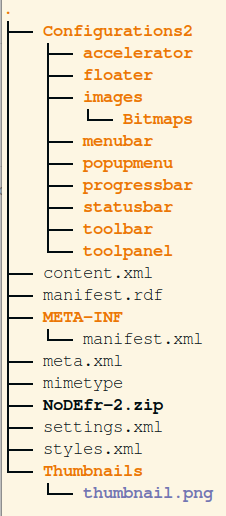
\includegraphics[scale=0.4]{arborescence.png}
%\caption{Arborescence!}
\end{columns}
\end{frame}

%%%%%%%%%%%%%%%%%%%%%%%%%%%%%%%%%%%%%%%%%%%%%%%%%%%%%%%%%%%%%%%%%%%%%%%%%%%%%%%%%%%%%%
\begin{frame}
\frametitle{Contextualisation}

\begin{figure}
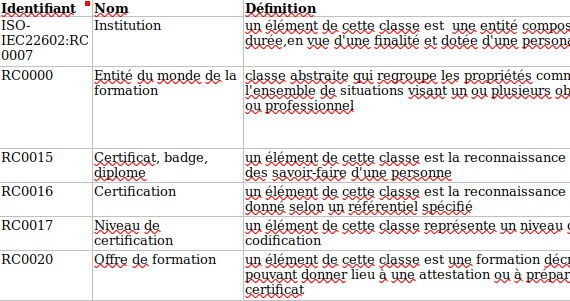
\includegraphics[scale=0.5]{extraitClasses.png}
\caption{Extrait de NoDEfr-2.ods}
\end{figure}
\end{frame}

%%%%%%%%%%%%%%%%%%%%%%%%%%%%%%%%%%%%%%%%%%%%%%%%%%%%%%%%%%%%%%%%%%%%%%%%%%%%%%%%%%%%%%
\begin{frame}[fragile]
\frametitle{Contextualisation}

Extrait du "content.xml" pour avoir un aperçu des balises :

\vspace{0.5cm}
\begin{lstlisting}[language=XML]
<table:table-cell table:style-name="ce67" office:value-type="string" calcext:value-type="string">
    <text:p>ISO-IEC22602:RC0007</text:p>
</table:table-cell>
<table:table-cell table:style-name="ce67" office:value-type="string" calcext:value-type="string">
    <text:p>Institution</text:p>
</table:table-cell>
<table:table-cell table:style-name="ce67" office:value-type="string" calcext:value-type="string">
    <text:p>un élément de cette classe est <text:s/>
une entité composée d&apos;êtres humains, organisée dans la durée,en vue d&apos;une finalité et dotée d&apos;une personalité juridique</text:p>
</table:table-cell>
\end{lstlisting}
\end{frame}


%%%%%%%%%%%%%%%%%%%%%%%%%%%%%%%%%%%%%%%%%%%%%%%%%%%%%%%%%%%%%%%%%%%%%%%%%%%%%%%%%%%%%%
\begin{frame}
\frametitle{Contextualisation}

\begin{figure}

\includegraphics[scale=0.5]{listeClasses.png}
\caption{Extrait de NoDEfr-2.ods}
\end{figure}
\end{frame}


%%%%%%%%%%%%%%%%%%%%%%%%%%%%%%%%%%%%%%%%%%%%%%%%%%%%%%%%%%%%%%%%%%%%%%%%%%%%%%%%%%%%%%
\begin{frame}[fragile]
\frametitle{Explication de notre implémentation}

Extrait de notre "NoDEfr-2.xsl" qui récupère le contenu des relations liées aux classes :

\vspace{0.5cm}
\begin{lstlisting}[language=XML]
<xsl:template match="table:table">
    <xsl:for-each select=".//table:table-row/following-sibling::table:table-row[1]">
        <xsl:element name="relation">
            <xsl:attribute name="identifiant">
                <xsl:value-of select=".//table:table-cell[1]/text:p"/>
            </xsl:attribute>
            <xsl:element name="nom">
                <xsl:value-of select=".//table:table-cell[2]/text:p"/>
            </xsl:element>
            <xsl:element name="definition">
                <xsl:value-of select=".//table:table-cell[3]/text:p"/>
            </xsl:element>
            <xsl:element name="indicateurLinguistique">
                <xsl:value-of select=".//table:table-cell[4]/text:p"/>
            </xsl:element>
            <xsl:element name="coDomaine">
                <xsl:value-of select=".//table:table-cell[5]/text:p"/>
            </xsl:element>
\end{lstlisting}
\end{frame}


%%%%%%%%%%%%%%%%%%%%%%%%%%%%%%%%%%%%%%%%%%%%%%%%%%%%%%%%%%%%%%%%%%%%%%%%%%%%%%%%%%%%%%
\begin{frame}[fragile]
\frametitle{Explication de notre implémentation}

Attribut qui indique le nombre de colonnes qui se répètent :

\vspace{0.5cm}
\begin{lstlisting}[language=XML]
<table:table-cell table:style-name="ce29" table:number-columns-repeated="3"/>
\end{lstlisting}

\begin{alertblock}{Difficulté}
\begin{itemize}
    \item Localisation de cette balise
    \item Création de boucles qui permet de créer un template assez générique
\end{itemize}
\end{alertblock}


\end{frame}



%%%%%%%%%%%%%%%%%%%%%%%%%%%%%%%%%%%%%%%%%%%%%%%%%%%%%%%%%%%%%%%%%%%%%%%%%%%%%%%%%%%%%%
\begin{frame}[fragile]
\frametitle{Explication de notre implémentation}

Extrait de notre "NoDEfr-2.xsl"

\vspace{0.5cm}
\begin{lstlisting}[language=XML]
<xsl:call-template name="regleDeContenu">
    <xsl:with-param name="j" select="6"/>
</xsl:call-template>
<xsl:variable name="repetition">
    <xsl:value-of select="number(.//table:table-cell[6]/@table:number-columns-repeated)"/>
</xsl:variable>

<xsl:choose>
    <xsl:when test="$repetition=4">
        <xsl:call-template name="raffine">
            <xsl:with-param name="j" select="6"/>
        </xsl:call-template>
        <xsl:call-template name="exemple">
            <xsl:with-param name="j" select="6"/>
        </xsl:call-template>
        <xsl:call-template name="note">
            <xsl:with-param name="j" select="6"/>
        </xsl:call-template>
        <xsl:call-template name="card_temp">
            <xsl:with-param name="i" select="7"/>
        </xsl:call-template>
    </xsl:when>
\end{lstlisting}
\end{frame}

%%%%%%%%%%%%%%%%%%%%%%%%%%%%%%%%%%%%%%%%%%%%%%%%%%%%%%%%%%%%%%%%%%%%%%%%%%%%%%%%%%%%%%
\begin{frame}[fragile]
\frametitle{Le fichier XML produit}

Première partie :

\vspace{0.5cm}
\begin{lstlisting}[language=XML]
<?xml version="1.0" encoding="UTF-8"?>
<Modele>
   <classe identifiant="RC0000">
      <nom>Entité du monde de la formation</nom>
      <definition>classe abstraite qui regroupe les propriétés communes à toutes les situations ou à l ensemble de situations visant un ou plusieurs objectifs de développement personnel ou professionnel</definition>
      <sousClasseDe/>
      <note>Super classe de toutes les classes. Elle regroupe toutes les propriétés des classes présentes dans ce modèle  </note>
\end{lstlisting}
\end{frame}


%%%%%%%%%%%%%%%%%%%%%%%%%%%%%%%%%%%%%%%%%%%%%%%%%%%%%%%%%%%%%%%%%%%%%%%%%%%%%%%%%%%%%%
\begin{frame}[fragile]
\frametitle{Le fichier XML produit}

Deuxième partie :

\vspace{0.5cm}
\begin{lstlisting}[language=XML]
<?xml version="1.0" encoding="UTF-8"?>
<Modele>
   <classe identifiant="RC0000">
      ...
      <relation identifiant="DES000001">
         <nom>libellé</nom>
         <definition>nommage humainement compréhensible de l élément</definition>
         <indicateurLinguistique>oui</indicateurLinguistique>
         <coDomaine>Littéral</coDomaine>
         <regleDeContenu>MLR String</regleDeContenu>
         <raffine/>
         <exemple>Pour une instance de la classe RC0020 Offre de formation, le libellé pourraît être " BTS services informatiques aux organisations"</exemple>
         <note/>
         <cardinaliteMinimale>1</cardinaliteMinimale>
         <cardinaliteMaximale>1</cardinaliteMaximale>
         <raison/>
      </relation>
\end{lstlisting}
\end{frame}

%%%%%%%%%%%%%%%%%%%%%%%%%%%%%%%%%%%%%%%%%%%%%%%%%%%%%%%%%%%%%%%%%%%%%%%%%%%%%%%%%%%%%%
\begin{frame}
\frametitle{Conclusion}

Merci pour votre attention !


\end{frame}

\end{document}